\subsection{Analiza systemów informatycznych z użyciem sieci Petriego}

\textbf{Sieci Petriego} – jest to matematyczna reprezentacja systemów rozproszonych. Umożliwiają one badanie zjawisk współbieżnych zachodzących w systemach wzajemnie się warunkujących w czasie. \textbf{Uogólniają one teorię automatów}.

\subsubsection{Definicja}

Podstawowa wersja sieci Petriego składa się z:

\begin{itemize}
	\item \textbf{miejsc} (odpowiadających warunkom),
	\item \textbf{przejść} (odpowiadających zdarzeniom),
	\item \textbf{łuków} (krawędzi, odpowiadających związkom między zdarzeniami i warunkami. \\
\end{itemize}

Aby opisać konkretny stan układu, potrzebne są żetony które można przemieszczać pomiędzy miejscami poprzez przejścia po krawędziach grafu. Oznaczeniami są:

\begin{itemize}
	\item \textbf{kropki} – żetony
	\item \textbf{prostokąty}(grube kreski) – przejścia
	\item \textbf{okręgi} – miejsca
	\item \textbf{strzałki} – krawędzie, łuki \\

\end{itemize}

Działanie sieci polega na przesuwaniu się znaczników między miejscami sieci.

\subsubsection{Własności sieci Petriego}

\begin{itemize}
	\item \textbf{Osiągalność} – sprawdzanie, czy dany stan jest osiągalny ze stanu początkowego (tzn. czy istnieje skończona liczba przejść, która prowadzi od znakowania początkowego do znakowania badanego).
	\item \textbf{Ograniczoność} – liczba znaczników w danym miejscu jest ograniczona.
	\item \textbf{Zachowawczość} – sieć Petriego jest zachowawcza, jeżeli liczba występujących w niej znaczników jest stała.
	\item \textbf{Żywotność} – określa liczbę możliwych wykonań przejścia. Sieć jest żywa, jeżeli z każdego oznakowania można osiągnąć inne oznakowania.
	\item \textbf{Odwracalność} – sieć jest odwracalna, jeżeli stan początkowy sieci jest osiągalny z każdego oznakowania.
\end{itemize}

\subsubsection{Analiza Sieci Petriego}

Trzy główne metody analizy sieci Petriego:

\begin{itemize}
	\item \textbf{Grafy osiągalności} – opiera się ona na budowie drzewa osiągalności. Ze stanu początkowego odpala się wszystkie możliwe przejścia , które prowadzą do osiągalnych znakowań tworzących węzły grafu, z nich tworzone są kolejne, itd. W drzewie osiągalności można w sposób jednoznaczny dojść od korzenia do dowolnego innego węzła. Drzewo może być nieskończone.
	\item \textbf{Grafy pokrycia} - otrzymywany jest z drzewa pokrycia poprzez scalenie duplikujących się wierzchołków. Na podstawie skończonego grafu pokrycia możliwe jest badanie sieci o nieskończonym zbiorze znakowań.
	\item \textbf{Metody algebraiczne} (macierz incydencji). Definiuje się macierz wejść wyjść. W macierzy incydencji liczba wierszy to liczba miejsc, liczba kolumn to liczba przejść.
\end{itemize}

\subsubsection{Przykład sieci Petriego}

Chcemy zaprojektować oprogramowanie dla systemu kontroli sygnalizacji świetlnej. Zakładamy, że dane są dwa autonomiczne systemy sterujące sygnalizacją świetlną – jeden dla pojazdów i drugi dla ludzi. Należy je zsynchronizować.

\begin{figure}[H]
	\centering
	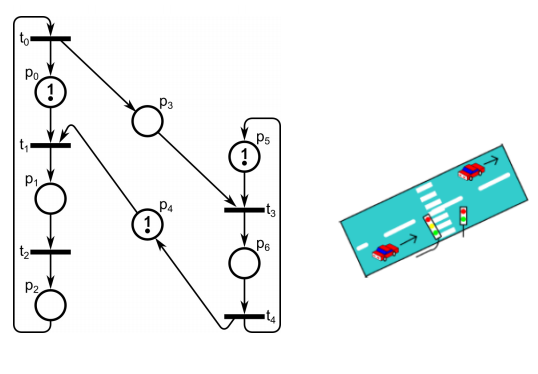
\includegraphics[width=0.6\linewidth]{K7.png}
	\caption{Przykładowa sieć}
\end{figure}

Znaczenie miejsc na powyższym rysunku jest następujące:

\begin{itemize}
	\item \textbf{$p_0$}, \textbf{$p_1$}, \textbf{$p_2$} – światła uliczne dla aut, odpowiednio $p_0$ – czerwone, $p_1$ – żółte, $p_2$ – zielone,
	\item \textbf{$p_3$}, \textbf{$p_4$} – miejsca służące do synchronizacji (np. flagi umieszczone w oprogramowaniu),
	\item \textbf{$p_5$}, \textbf{$p_6$} – światła uliczne dla pieszych, odpowiednio $p_5$ – czerwone, $p_6$ – zielone
\end{itemize}

\subsubsection{Formalny Opis powyższej sieci}

\begin{align*}
SP = &\langle P, T, F, H, W, C, M_0\rangle \\
P = &\{p_0, p_1, p_2, p_3, p_4, p_5, p_6\} \\
T = &\{t_0, t_1, t_2, t_3, t_4 \} \\
F =  &\big\{ 
\{p_0, t_1\}, \{t_1, p_1\}, \{p_1, t_2\}, \{t_2, p_2\},\{p_2, t_0\}, \{t_0, p_0\},  \{t_0, p_3\}, \\
&\{p_3, t_3\}, \{t_3, p_6\}, \{p_6, t_4\}, \{t_4, p_5\}, \{p_5, t_3\}, \{t_4, p_4\}, \{p_4, t_1\}         \big\} \\
H =  &\emptyset \\
W = &\big\{ 1, 1, ... , 1\big\} \\
C = &\big\{ \infty, \infty, ... , \infty \big\} \\
M_0 = &\big\{ p_0 = 1, p_4 = 1, p_5 = 1 \big\}
\end{align*}

, gdzie:
\begin{multicols}{2}
	\begin{itemize}[nolistsep]
		\item $SP$ - sieć Petriego
		\item $P$ - zbiór miejsc
		\item $T$ - zbiór przejść
		\item $F$ - zbiór łuków zwykłych
	\end{itemize}
	\columnbreak
	\begin{itemize}[nolistsep]
		\item $H$ - zbiór łuków hamujących
		\item $W$ - wagi łuków
		\item $C$ - pojemność miejsc
		\item $M_0$ - znakowanie początkowe
	\end{itemize}
\end{multicols}

\subsubsection{Graf osiągalności powyższej sieci}

\begin{figure}[H]
	\centering
	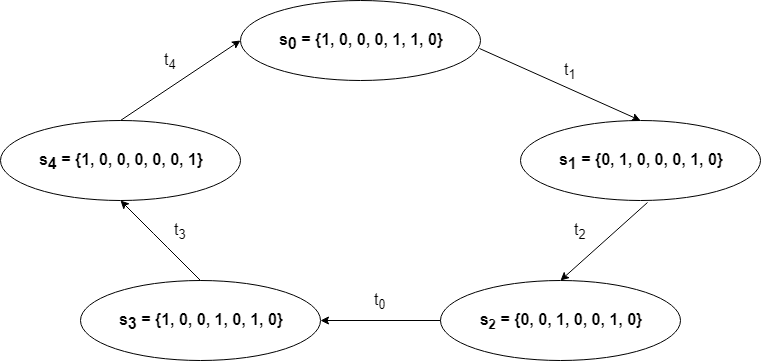
\includegraphics[width=0.6\linewidth]{K7_1.png}
	\caption{Przykładowy graf osiągalności}
\end{figure}

\subsubsection{Analiza behawioralna}

\begin{itemize}
	\item \textbf{Ograniczoność sieci} \\
	\textbf{Jest} ograniczona (1-ograniczona), co łatwo zauważyć na grafie osiągalności. Dla każdego znakowania w każdym miejscu znajduje się co najwyżej jeden znacznik. 
	\item \textbf{Bezpieczeństwo sieci} \\
	Analizowana sieć \textbf{jest} bezpieczna, ponieważ jest 1-ograniczona(patrz punkt wyżej).
	\item \textbf{Zachowawczość sieci} \\
	Badana sieć \textbf{nie jest} zachowawcza. Liczba znaczników w poszczególnych stanach zmienia się od 2 do 3.
	\item \textbf{Żywotność sieci} \\
	Sieć z \textbf{jest} żywotna, ponieważ w każdym jej osiągalnym stanie można odpalić przynajmniej jedno przejście i każde jej przejście może być kiedyś odpalone.
	\item \textbf{Odwracalność}  \\
	sieć \textbf{jest} odwracalna, stan początkowy sieci jest osiągalny z każdego oznakowania.
\end{itemize}
